\chapter{ADT, List, Stack and Queue}

\section{Abstract Data Type (ADT)}
We use data abstraction to simplify software development since it facilitates the decomposition of the complex task of developing a software system. To put it simply, data abstraction shows only the essential details of data, while the implementation details are hidden.

For example, as will be discussed later, List, Stack, and Queue (LSQ) are forms of data abstraction, or what we call abstract data types. We can use them to retrieve or store data, but we don't know how they are actually stored or indexed.

Data encapsulation, or information hiding, is the concealing of the implementation of a data object from the outside world. Through data abstraction, we can separate the specification of a data object from its implementation.

A data type is a collection of objects and a set of operations that act on those objects. An abstract data type (ADT) is a data type organized in such a way that we can separate the specification of the object and the specification of the operations on the object. Abstract data types are simply a set of operations, and they are mathematical abstractions.

Note that abstraction is like a functional description without knowing how to use it, while implementation, on the contrary, is something that can be used and executed.

In summary, an ADT is a high-level description of how data is organized and the operations that can be performed on it. It abstracts the details of its implementation and only exposes the operations that are allowed on data structures.

\section{List}
The first abstract data type in this chapter is List.

\subsection{Overview}
When dealing with a general list of the form \(a_1, a_2, \cdots, a_n\), we say that the size of this list is \(n\). If the list is of size 0, we call it the \textbf{null list}. Except null list, we say that \(a_{i+1}\) follows/succeeds \(a_i (i < n)\) and that \(a_{i-1}\) precedes \(a_i (i > 1)\). 

The first element of the list is \(a_1\), and the last element is \(a_n\). The predecessor of \(a_1\) and the successor of \(a_n\) is not defined. 

\subsection{Operations}
A list of elements of type \(T\) is a finite sequence of elements of \(T\) together with the following operations:

- Create the list and make it empty.

- Determine whether the list is empty or not.

- Determine whether the list is full or not.

- Find the size of the list.

- Retrieve any entry from the list, provided that the list is not empty.

- Store a new entry, replacing the entry at any position in the list, provided that the list is not empty.

- Insert a new entry into the list at any position, provided that the list is not full.

- Delete any entry from the list, provided that the list is not empty.

- Clear the list to make it empty.

With these operations, we can perform various tasks on the list ADT.

\subsection{Complexity}
We can use an array to implement a list. Most of the operations follow linear time, for example, \verb|print_list|, \verb|make_null|, \verb|find|, and \verb|find_kth|. For insertion, there could be cases where the list is full, and that's why we need dynamically allocated space. For deletion, we need to find the element, perform the deletion, and reallocate space, which might require more time. Thus, we introduce the linked list.

\subsection{Linked List}
There are several types of linked lists:

- Singly Linked List  
{\par\centering
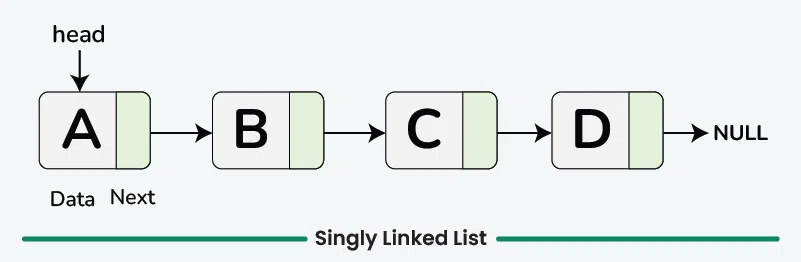
\includegraphics[width=0.4\textwidth]{Figure/singly-linked-list.png}
\par}

- Singly Linked List with Header  
{\par\centering
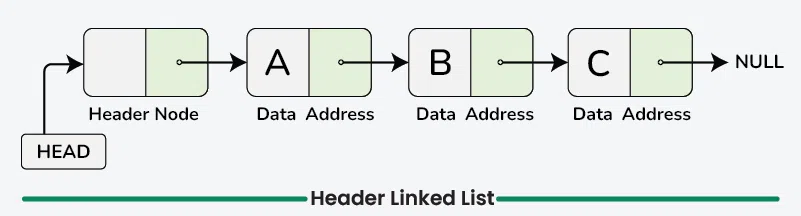
\includegraphics[width=0.4\textwidth]{Figure/header-linked-list.png}
\par}

- Doubly Linked List  
{\par\centering
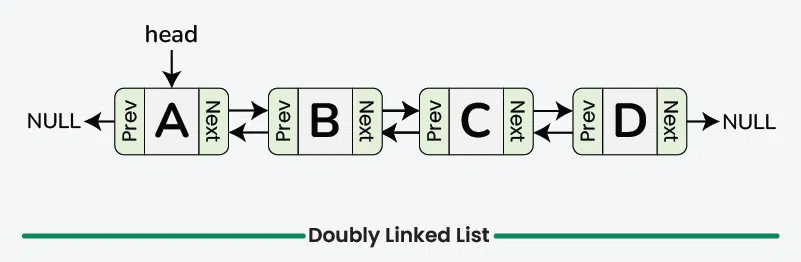
\includegraphics[width=0.4\textwidth]{Figure/doubly-linked-list.png}
\par}

- Circularly Linked List  
{\par\centering
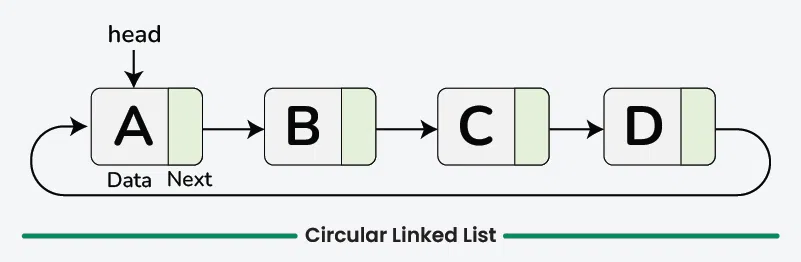
\includegraphics[width=0.4\textwidth]{Figure/circular-linked-list.png}
\par}

- Circularly Doubly Linked List  
{\par\centering
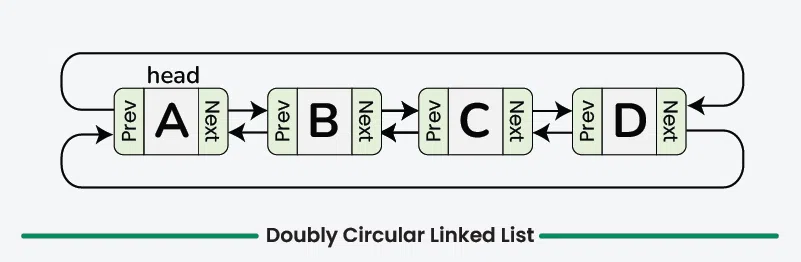
\includegraphics[width=0.4\textwidth]{Figure/double-cir-linked-list.png}
\par}

A polynomial can be represented as
\[
  F(X) = \sum_{i = 0}^N A_{i} X^i
\]
For example, \(F(X) = 4X^3 + 2X^2 + 5X + 1\). We may want to perform operations like addition, subtraction, multiplication, and differentiation. Using an array data structure, the time complexity may be larger due to the need to store all terms, including zero coefficients. However, with a linked list, we can efficiently perform these operations by traversing the linked list and processing only the non-zero terms.

Also, note that a circular list saves space but not time. It is useful for smaller datasets. However, for a larger number of students and courses, the use of such a circular list might be a waste of space.

In summary, a list abstract data type represents an ordered collection of elements. They can be added or removed at any position in the list. It provides methods to access elements by their position.

By using different types of linked lists, we can achieve various goals. For example, we can print all the elements in reverse using a doubly linked list.

\section{Stack}





\section{Queue}